\chapter{Аналитический обзор}
\label{cha:analysis}
%
% % В начале раздела  можно напомнить его цель
%
%В данном разделе анализируется и классифицируется существующая всячина и пути создания новой всячины. А вот отступ справа в 1 см. "--- это хоть и по ГОСТ, но ведь диагноз же...

%%%%%%%%%%%%%%%%%%%%%%%%%%%%%%%%%%%%%%%%%%%%%%%%%%%%%%%%%%%%%%%%%%%%%%%%%%%%%%%%%%%%%%%%%%%%%%%%%%%%%%%%%%%%%%%%

\section{Что такое Интернет вещей}

Интернет вещей (англ. \textit{IoT}, \textit{Internet of Things}) ""--- это методология вычислительной сети физических объектов (``\textit{вещей}''), имеющих встроенную поддержку технологий передачи данных для их взаимодействия, а также для взаимодействия с внешней средой.
Эта методология рассматривает Интернет вещей как явление, способное перестроить культурные и экономические процессы, всё больше исключая человека из них.
Влияние существующего Интернета на сферы образования, коммуникации, бизнеса, науки и политики позволяет говорить о том, что Интернет является одним из важнейших и мощнейших изобретений в истории человечества\cite{evans2011internet}.
Интернет вещей стоит рассматривать как новую ветвь эволюции Интернета, где каждый предмет в поле зрения человека может быть оснащён датчиками, сенсорами, устройством управления и модулем передачи данных для общения со всем миром.

Как известно, большинство великих изобретений человечества потребовали десятки и даже сотни лет на переход от простых по форме представлений до сложных систем.
От создания предпосылок, до массового внедрения Интернета ушло почти четверть века, однако похоже что для Интернета вещей на то же самое потребуется существенно меньше времени \cite{chernyak2013}.
Международный союз связи (МСЭ) и Европейский Союз определили Интернету вещей главенствующую роль в дальнейшем развитии отрасли инфокоммуникации. 
По расчетам консалтингового подразделения Cisco IBSG (см. рис. \ref{fig:iotandpeople}) в промежутке между 2008 и 2009 годами, количество устройств, подключенных к интернету, превысило количество людей, и к 2020 году количество подключенных устройств достигнет 50 миллиардов\cite{evans2011internet} (по другим данным\cite{denise2014} ""--- 25 миллиардов).
Таким образом, в настоящее время происходит переход от ``Интернета людей'' к ``Интернету вещей''.
Хотя данная концепция на международном уровне уже обретает черты сформировавшейся технологии, для неё ведутся активные работы в области стандартизации компонентов, архитектуры и приложений.
Количество мнений о том как будет построен Интернет вещей очень велико. 
Это подтверждается большим разнообразием предлагаемых технологий для создания LPWAN сетей на рынке.

\begin{figure}
  \centering
  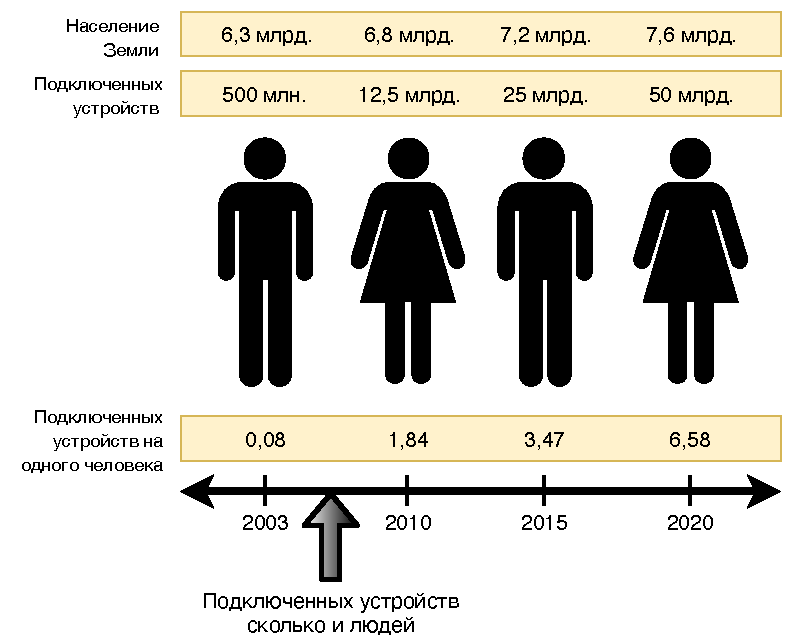
\includegraphics[width=0.8\textwidth]{inc/img/IoTAndPeople.pdf}
	\caption{Временная шкала изменения количества людей и предметов, подключенных к интернет \cite{evans2011internet}}
  \label{fig:iotandpeople}
\end{figure}

%Кстати, про картинки. Во-первых, для фигур следует использовать \texttt{[ht]}. Если и после этого картинки вставляются <<не по ГОСТ>>, т.е. слишком далеко от места ссылки, "--- значит у вас в РПЗ \textbf{слишком мало текста}! Хотя и ужасный параметр \texttt{!ht} у окружения \texttt{figure} тоже никто не отменял, только при его использовании документ получается страшный, как в ворде, поэтому просьба так не делать по возможности.

\subsection{Базовые принципы Интернета вещей}

Интернет вещей основывается на трёх базовых принципах\cite{roslyakov2014}.
\begin{enumerate}
	\item повсеместно распространенная инфраструктура;
	\item глобальная идентификация каждого объекта;
	\item возможность каждого физического объекта отправлять и получать данные, посредством локальной сети или сети Интернет, к которой он подключен.
\end{enumerate}

Наиболее важными отличиями Интернета вещей от интернета людей являются:
\begin{itemize}
	\item фокус на считывание информации, а не на коммуникациях;
	\item на порядки большее число подключенных к сети объектов;
	\item потребность в создании новых стандартов;
	\item намного меньше размеры объектов и скорости передачи данных;
	\item фокус не на человеке, а на вещах;
\end{itemize}

Концепция сетей следующего поколения NGN предполагала возможность коммуникаций людей в любой точке пространства и времени.
Концепция интернета вещей включает ещё одно направление ""--- коммуникация любых вещей или устройств (рис. \ref{fig:iotconcept})

\begin{figure}
  \centering
  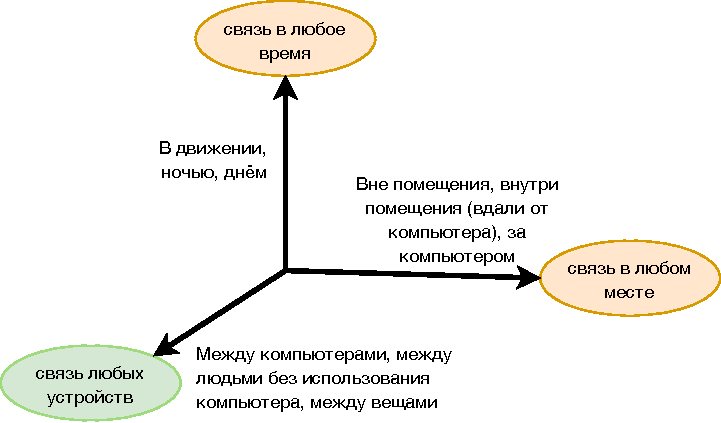
\includegraphics[width=0.8\textwidth]{inc/img/IoTConcept.pdf}
	\caption{Новое направление коммуникаций, реализуемой Интернетом вещей\cite{itutiot2012}}
  \label{fig:iotconcept}
\end{figure}

Согласно принятым в МСЭ-Т представлениям о отображении физических и виртуальных вещей, виртуальные вещи могут обходится без их физического соответствия, в то время как каждой физической вещи соответствует минимум один объект в виртуальном пространстве (см. рис. \ref{fig:physvirtworld}).  

Рекомендация Y.2060 от МСЭ-Т описывает различное сочетание способов соединений.
МСЭ-Т рассматривает множество сетевых технологий, как потенциально пригодных для приложений Интернета вещей, а именно: глобальные сети, локальные сети, ячеистые (mesh) сети и беспроводные самоорганизующиеся (ad-hoc) сети.

\begin{figure}
  \centering
  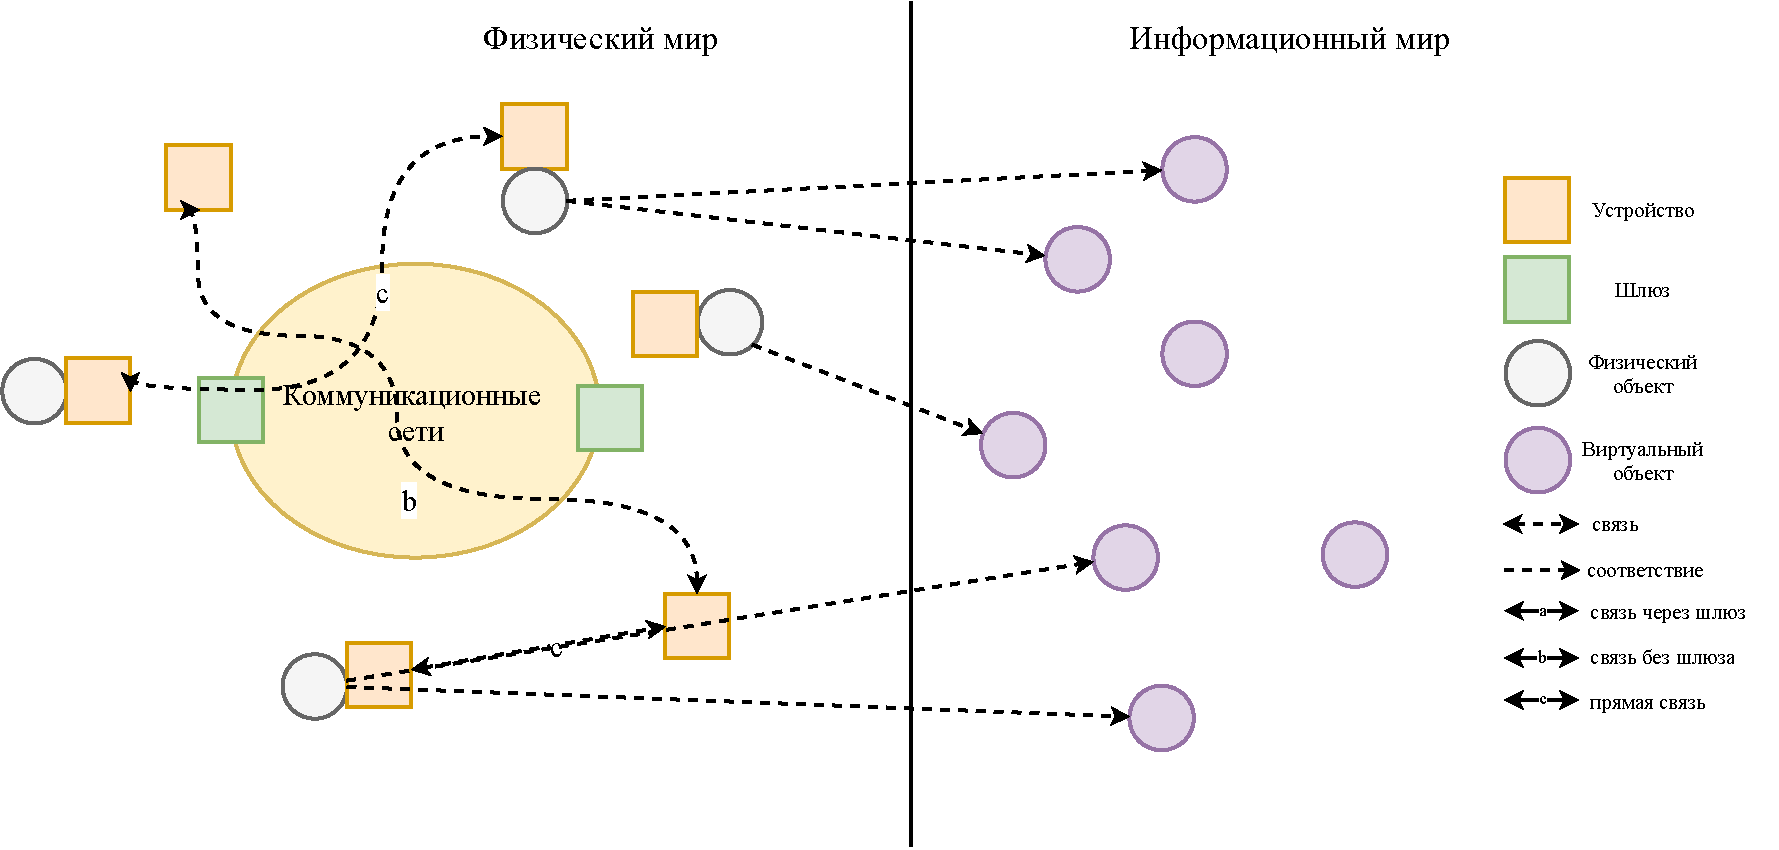
\includegraphics[width=0.9\textwidth]{inc/img/realvirtualthings}
	\caption{Отображение физических и виртуальных вещей\cite{itutiot2012}}
  \label{fig:physvirtworld}
\end{figure}

\subsection{Основные характеристики Интернета вещей}

IoT, имеет следующие характеристики:

\begin{itemize}
	\item возможность установления соединений. Любую вещь можно соединить к Интернету вещей;
	\item гетерогенность: устройства в концепции Интернета вещей являются гетерогенными и базируются на различных аппаратных платформах и сетях. 
		Могут обмениваться информацией с другими устройствами, независимо от структуры сети и применяемых технологий транспортного уровня. 
		Примечательно, что современное состояние сети Интернет может удовлетворить этому лишь отчасти: пул адресов IPv4 исчерпан и большая часть устройств скрывается в локальных сетях за устройствами NAT, что противоречит изначальной концепции однородного интернета. 
		Решением может стать повсеместное использование протокола IPv6 в качестве протокола сетевого уровня. 
		Хотя внедрение этого протокола и затянулось, но уже к декабрю 2018 года ожидается, что 25\% всех Интернет доменов будет доступно через этот протокол\cite{pickard2017}.;
	\item огромное количество, одновременно подключенных, устройств к сети, которыми необходимо управлять, обмениваться данными. Произойдёт существенное увеличение долей обмена данными, инициированными устройствами, по сравнению с долей информационного обмена, инициированного людьми;
	\item динамические изменения структуры сети. Устройства будут свободно подключаться к сетям, менять своё местоположение, отключаться от сети и подключаться к новым устройствам. Подразумевается, что количество устройств в одной сети - переменная величина с течением времени;
\end{itemize}

Важной частью рекомендации от МСЭ-Т являются требования	предъявляемые к устройствам IoT. Любые технологии LPWAN, в том числе и LoRa, должны соответствовать этим требованиям для предоставления возможности их включения в инфраструктуру Интернета вещей:

\begin{itemize}
	\item предоставление автономных услуг: требуется что бы услуги могли предоставляться с помощью автоматической передачи, обработки и сбора данных вещей, основанных на правилах, задаваемых операторами или абонентами. Услуги могут зависеть от методов автоматизированной обработки и интеллектуального анализа данных;
	\item соединение на основе идентификатора: соединение с любой вещью в концепции Интернета вещей будет происходить на основе уникального идентификатора, которым обладает тот или иной объект. Отсюда выходит требование о создании универсального идентификатора (например адрес IPv6) для применения в гетерогенных сетях.
	\item функциональная совместимость: требуется обеспечение функциональной совместимости гетерогенных и распределенных систем в целях предоставления и потребления самый разных видов услуг;
	\item  возможности определения местоположения: требуется что бы в Интернете вещей обеспечивались услуги, на основе информации о местоположении объекта. Требуется что бы информация о местоположении вещей отслеживалась автоматически. Связь и услуги на основе местоположения могут быть ограничены законами и нормативными актами и должны соответствовать требованиям безопасности;
	\item безопасность в Интернете вещей: каждая вещь имеет соединение с сетью, что приводит к серьёзной угрозе безопасности, таким как угроза аутентичности, целостности и конфиденциальности как данных, так и услуг. Одним и важнейших требования к безопасности является необходимость объединения различных методов и принципов обеспечения безопасности множества устройств и сетей пользователей;
	\item защита неприкосновенности частной жизни: требуется, чтобы в IoT обеспечивалась неприкосновенность частной жизни. У многих вещей есть владельцы и эти вещи могут хранить личную информацию их владельцев. Необходимо обеспечить неприкосновенность частной жизни человека при сборе, обработке, анализе и передачи больших массивов информации вещами. Защита неприкосновенности частной жизни не должна служить препятствием для аутентификации источника данных;
	\item автоматическое конфигурирование: необходимо обеспечить возможность автоматического конфигурирования устройств, для возможности оперативной модификации программного обеспечения вещей, с целю повысить качество обслуживания клиентов, а также степень интеграции устройства с окружающим миром и сетью, не нарушая при этом, требования о безопасности и конфиденциальности.
	\item управляемость: возможность вмешательства человека в работу вещей при необходимости.
\end{itemize}

\subsection{Эталонная модель Интернета вещей}

Также была разработана эталонная модель интернета вещей, она показана на рисунке \ref{fig:iotetalon}.
Она включает в себя четыре уровня, а также возможности обеспечения безопасности и управления, которые связаны с этими четырьмя уровнями:

\begin{itemize}
	\item уровень приложения;
	\item уровень поддержки услуг и поддержки приложения;
	\item уровень сети;
	\item уровень устройства.
\end{itemize}

\begin{figure}
  \centering
  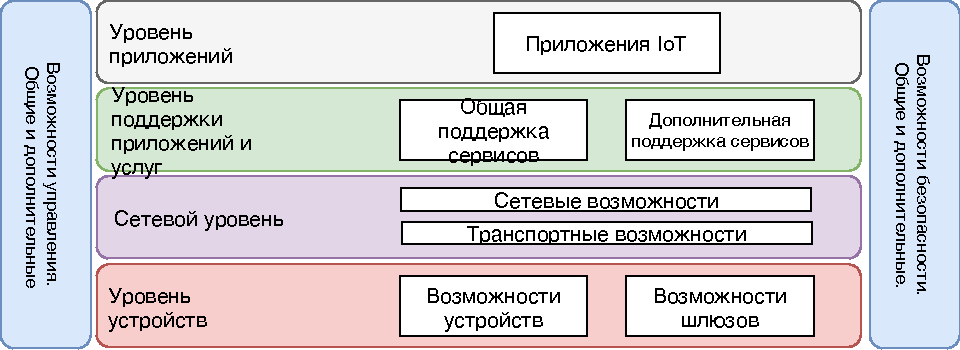
\includegraphics[width=\textwidth]{inc/img/IoTEtalon.pdf}
	\caption{Эталонная модель IoT\cite{itutiot2012}}
  \label{fig:iotetalon}
\end{figure}

%%%%%%%%%%%%%%%%%%%%%%%%%%%
%%%%%%%%%%%%%%%%%%%%%%%%%%%

\subsubsection{Уровень приложения}

Содержит само приложение IoT.

%%%%%%%%%%%%%%%%%%%%%%%%%%%
%%%%%%%%%%%%%%%%%%%%%%%%%%%

\subsubsection{Уровень поддержки услуг и поддержки приложений}

Данный уровень состоит из следующих двух групп возможностей:

\begin{itemize}
	\item общие возможности поддержки, или типовые возможности, которые могут использоваться приложениями Интернета вещей, такими как хранение или обработка данных.
	\item специализированные возможности поддержки или набор конкретных возможностей, предназначенных для удовлетворения требований разнообразных приложений.
\end{itemize}


%%%%%%%%%%%%%%%%%%%%%%%%%%%
%%%%%%%%%%%%%%%%%%%%%%%%%%%

\subsubsection{Уровень сети}

Существует два типа возможностей:

\begin{itemize}
	\item возможности организации сетей: предоставляет функции управления сетевыми соединениями;
	\item возможности транспортировки: предназначены для предоставления соединений для транспортировки информации в виде данных, относящихся к услугам и приложениям IoT, а также транспортировки информации управления и контроля, относящейся к IoT.
\end{itemize}

%%%%%%%%%%%%%%%%%%%%%%%%%%%
%%%%%%%%%%%%%%%%%%%%%%%%%%%

\subsubsection{Уровень устройства}

Этот уровень можно логически разделить на два вида возможностей:
\begin{itemize}
	\item возможности устройства. Это могут быть такие возможности, как: спящий режим и пробуждение, организация специальных сетей, прямое и непрямое взаимодействие устройства с сетью;
	\item возможности шлюза. Это возможность поддержки различных интерфейсов. Шлюза объединяют в себе различные сетевые интерфейсы, как проводные, так и беспроводные.
\end{itemize}

%%%%%%%%%%%%%%%%%%%%%%%%%%%
%%%%%%%%%%%%%%%%%%%%%%%%%%%

\subsubsection{Возможности управления}

Возможности управления IoT охватывают традиционные классы конфигурации, учета, безопасности и т.д.

Важнейшие возможности управления включают:
\begin{itemize}
	\item управление устройствами, диагностика, обновление, прошивка, управление рабочим состоянием устройства;
	\item управление топологией локальной сети;
	\item управление трафиком и перегрузками.
\end{itemize}

\subsubsection{Возможности обеспечения безопасности}

Есть два вида возможностей обеспечения безопасности: общие и специализированные.
Общие возможности не зависят от приложений и включают:
\begin{itemize}
	\item на уровне приложений: авторизацию, конфиденциальность, аутентификацию, целостность данных приложения, защиту неприкосновенности частной жизни, аудит безопасности;
	\item на уровне сети: авторизацию, аутентификацию, защиту конфиденциальности и целостности;
	\item на уровне устройства: аутентификацию, авторизацию, проверку целостности устройства, управление доступом, защиту целостности и конфиденциальности.
\end{itemize}

Специализированные возможности зависят от вида приложений и могут налагать дополнительные специфичные требования по безопасности.

%%%%%%%%%%%%%%%%%%%%%%%%%%%%%%%%%%%%%%%%%%%%%%%%%%%%%%%%%%%%%%%%%%%%%%%%%%%%%%%%%%%%%%%%%%%%%%%%%%%%%%%%%%%%%%%%
\newpage
\section{Обзор технологии LoRa} 

LoRa представляет собой технологию энергоэффективной сети дальнего радиуса действия, разрабатываемый организацией LoRa Alliance.
Данная технология нацелена на использование в устройствах с автономными источниками питания, где показатель энергопотребления является наиболее важным.
В данном разделе будет дан обзор на данную технологию.
Будет кратко рассмотрены физический и уровень управления доступом к сети (MAC) LoRaWAN сетей.

\subsubsection{Стек протоколов LoRa}

На рисунке \ref{fig:lorastack} изображён стек протоколов в сетях LoRaWAN. 

\begin{figure}[!h]
  \centering
  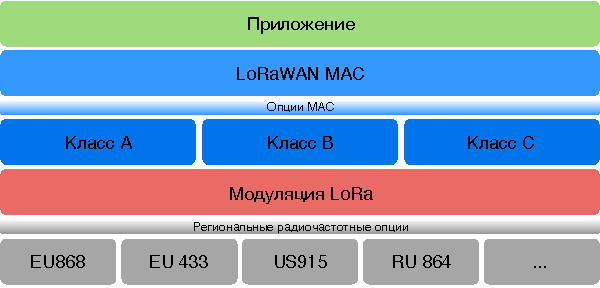
\includegraphics[width=0.9\textwidth]{inc/img/LoRaStack.pdf}
	\caption{Стек протоколов LoRaWAN}
  \label{fig:lorastack}
\end{figure}

Далее будут кратко рассмотрены все уровни данного стека протоколов.

\subsubsection{Сетевая архитектура LoRa}

Стандартной топологией LoRa является ``звезда из звёзд'', которая включает в себя различные типы устройств, как показано на рисунке \ref{fig:loranetworkarch}.

\begin{figure}[ht]
  \centering
  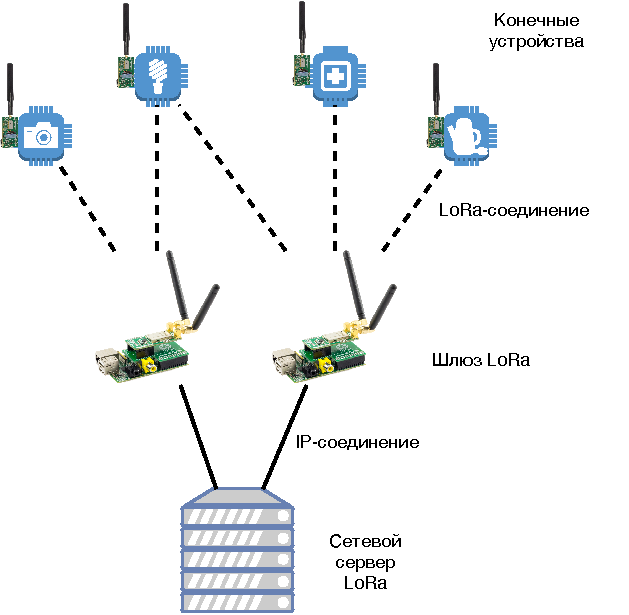
\includegraphics[height=0.4\textheight]{inc/img/LoRaNetworkArch.pdf}
  \caption{Сетевая архитектура LoRa}
  \label{fig:loranetworkarch}
\end{figure}

%%%%%%%%%%%%%%%%%%%%%%%%%%%
\subsection{Физический уровень}

Технология LoRa описывает два независимых уровня протоколов: физический, с использование линейной частотной модуляцией (CSS); и протокол контроля доступа к среде (LoRaWAN), хотя системы коммуникации LoRa также реализуют специфичные сетевые архитектуры\cite{augustin2016}.

Физический уровень LoRa разработан компанией Semtech и он обеспечивает связь с низким энергопотреблением, низкой скоростью и большим радиусом действия.
Размер полезных данных может изменятся в диапазоне от 2 до 255 октетов, а скорость передачи данных может достигать до 50 Кбит/c. 
Технология модуляции закрыта и является собственностью компании Semtech, поэтому здесь будут рассмотрены только известные принципы работы передатчиков и приёмников LoRa.

LoRa использует линейную частотную модуляцию, которая использует линейное изменение частоты несущей во время передачи закодированной информации.
Благодаря линейному возрастанию частоты сигнала смещение частоты между приёмником и передатчиком за промежуток времени передачи символа остаётся постоянным, что легко устраняется демодулятором\cite{augustin2016}. 
Это делает данную модуляцию невосприимчивой к эффекту Доплера.
Смещение частот между приёмником и передатчиком может достигать 20\% ширины полосы частот без влияния на корректность демодуляции.
Это помогает уменьшить стоимость приёмников и передатчиков LoRa, поскольку смягчены требования на точность встроенных кварцевых резонаторов.
Все эти особенности делают возможным для приёмников LoRa приём сигнала мощностью до -130 dBm.

\subsubsection{Параметры физического уровня} 

Есть несколько параметров для настройки модуляции LoRa: 
\begin{enumerate}
	\item полоса пропускания (\textit{BW}); 
	\item коэффициент расширения спектра (\textit{SF}); 
	\item кодовая скорость (\textit{CR}).
\end{enumerate}

Также могут быть изменены следующие настройки радиомодулей:
\begin{itemize}
	\item длина преамбулы, значение синхронизирующего слова SyncWord;
	\item посылать ли явно заголовок с сообщением, он содержит информацию о параметрах приёма остальной части сообщения (длина полезных данных, параметр CR и наличие CRC);
	\item наличие поля CRC;
	\item бит LowDataRateOptimization (DE).
\end{itemize}

\subsubsection{Модуляция и кодирование}

\paragraph{Радиосигнал с линейной частотной модуляцией (ЛЧМ)} \hspace{0pt}\\

Физический радиоинтерфейс LoRa использует широкополосные сигналы с линейной частотной модуляцией\cite{augustin2016}. 
ЛЧМ ""--- давно известная технология, применявшаяся в радиолокации, но в качестве основы кодирования цифровых данных использовалась реже.
При линейной модуляции частота сигнала испытывает линейную девиацию (возрастает или уменьшается) со временем. 
Частота изменяется в пределах ширины канала частот (с англ. \textit{Bandwith, BW}), таким образом, она изменяется по закону:
\begin{equation}
	\omega(t) = \omega_0 + \mu t
\end{equation}

Здесь $\omega_0$ - несущая частота; $\mu$ - параметр с размерностью с$^{-2}$, равный скорости изменения частоты во времени.

За время, равное длительности импульса, девиация частоты равна
\begin{equation}
	\Delta \omega = \mu \tau_{\text{и}},
\end{equation}

где $\tau_{\text{и}}$ ""--- длительность сигнала, а полная фаза сигнала:
\begin{equation}
	\psi(t) = \omega_0 + \mu t{^2}/2
\end{equation}

Сигнал ЛЧМ представляется следующей математической моделью\cite{Baskakov2003}:
\begin{equation}
	u_\text{ЛЧМ}(t) = 
	\begin{cases}
		0, & t < -\tau_\text{и}/2,\\
		U_m cos(\omega_0 t + \mu t{^2}/2), & -\tau_\text{и}/2 \le t \le \tau_\text{и}/2,\\
		0, & t > \tau_\text{и}/2.
	\end{cases}
\end{equation}

Анализ характера частотной зависимости модуля и фазы спектральной плотности прямоугольного ЛЧМ-импульса выявил\cite{Baskakov2003} полную зависимость от безразмерного числа:
\begin{equation}
	B = \Delta f \tau_\text{и} = \mu \tau^{2}_{\text{и}}/(2\pi),
\end{equation}

равного произведению девиации частоты на длительноть импульса, называемого \textit{базой} ЛЧМ-сигнала.

На практике обычно стараются выполнить условие $B \gg 1$. 
Спектр таких ЛЧМ-сигналов имеет ряд особенностей, и одной из них является то, что модуль спектральной плотности практически постоянен в пределах полосы частот шириной $\Delta \omega$ с центром в точке $\omega_0$.
В LoRa этим параметром косвенно манипулируют за счёт увеличения коэффициента расширения спектра (\textit{Spreading Factor}, \textit{SF}).
SF ""--- это логарифмический параметр, соответствующий продолжительности передачи одного символа:
\begin{equation}
	B = \Delta f \tau_\text{и} = 2^{SF}
\end{equation}

Значение SF может варьироваться от 6 до 12.

LoRa кодирует символы циклическим сдвигом чирпа относительно кадра времени. 
Скачок фазы и обозначает кодируемый символ.
Поскольку $2^{SF}$ чирпов могут находится в символе, то и один символ может эффективно кодировать SF бит информации.

Пропускная способность чирпов зависит только от ширины полосы частот.
Увеличение SF повлечет за собой деление продолжительности чирпа на два (поскольку $2^{SF}$ чирпов покрывают всю ширину полосы частот) и увеличением в два раза продолжительности передачи символа.
Пропускная способность не уменьшиться в два раза, поскольку теперь каждый символ кодирует на один бит больше.

Также LoRa реализован механизм прямой коррекции ошибок (\textit{Forward Error Correction}, \textit{FEC}).
Параметр CR может быть равен $4/(4+n)$, где $n \in \{1, 2, 3, 4\}$.
Принимая это во внимание, можно вычислить полезную пропускную способность по формуле \ref{formula:rb}.
\begin{equation}
 R_b = SF \frac{\Delta f}{2^{SF}} CR \label{formula:rb}
\end{equation}

Для примера, если имеем $\Delta f$ (Он же BW) = 125 кГц, SF = 8, CR = $4/8$, то получаем полезную пропускную способность равную 1,95 Кбит/с.
Все вышеприведенные особенности позволяют добиться высокой помехозащищённости и, как следствие, большой зоны покрытия сети.

Пример сигнала, принятым анализатором спектра от передатчика LoRa, изображен на рисунке \ref{fig:loradecoding}.

\begin{figure}[!h]
  \centering
  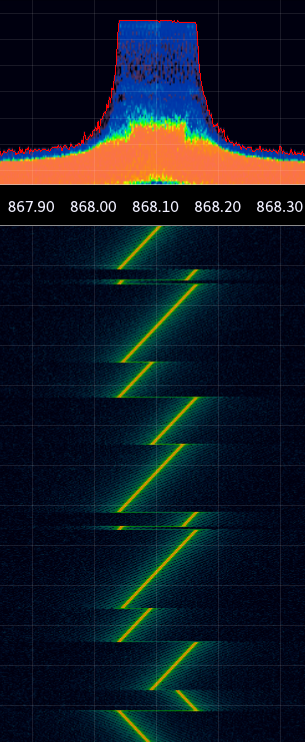
\includegraphics[height=0.4\textheight]{inc/img/LoRaDecoding}
  \caption{Сигнал LoRa (внизу) и его спектр (вверху)\cite{DecodingLora2018}}
  \label{fig:loradecoding}
\end{figure}

\subsubsection{Формат кадра физического уровня}\label{part:physframe}

Хотя модуляция LoRa позволяет отправлять произвольные кадры, формат кадра физического уровня был описан и реализован в передатчика и приёмниках от Semtech.
Ширина полосы частот и коэффициент расширения спектра не изменяются в рамках кадра.

Кадр LoRa начиначется с преамбулы (см. рис. \ref{fig:loraphysframe}): последовательности растущих чирпов, занимающих всю частотную полосу.
Два последних чирпа кодируют синхронизирующее слово.
Синхронизирующее слово это одно-байтовое значение, которое используется для опознания двух разных сетей, использующих один и тот же канал для связи. 
Устройство, сконфигурированное на приём заданного слова синхронизации остановит приём данных если принятое слово синхронизации не совпало с заданным.
Слово синхронизации следует за двумя или четырьмя спадающими чирпами в преамбуле.
Длина преамбулы может быть изменено между 10,25 и 65539,25 символами.

Когда после преамбулы задаётся необязательный заголовок, он кодируется и передаётся с CR = $4/8$.
Он указывает на размер полезной нагрузки (в байтах), CR используемое для кодирования и наличие необязательного 16-битного поля CRC.
CRC (если оно есть) находится в конце кадра, сразу после полезной нагрузки.
Поле размера полезной нагрузки имеет размер в один байт, что ограничивает максимальный размер полезной нагрузки в 255 байт.

\begin{figure}[!h]
  \centering
  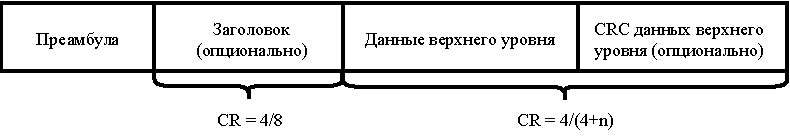
\includegraphics[width=\textwidth]{inc/img/LoRaPhysFrame.pdf}
  \caption{Структура кадра физического уровня LoRa}
  \label{fig:loraphysframe}
\end{figure}

%Поддерживаемые радиоинтерфейсом LoRa значения BW: 125, 250, 500 кГц.

\subsubsection{Доступные частотные диапазоны}

Физический уровень LoRa работает в различных субгигагерцовых частотных ISM диапазонах.
В различных странах приняты различные диапазоны частот, поэтому устройствам с LoRa необходимо самостоятельно выбирать используемый радиодиапазон для физического уровня, в зависимости от принятых местных соглашениях. 
Таблица \ref{tab:ismbands} описывает, принятые в различных странах, частотные диапазоны для строительства сетей связи.

\begin{table}[ht]
  \caption{частотные диапазоны, принятые в разных странах}
  \begin{tabular}{|l|c|}
  \hline
	  Частотный диапазон & Страна\\
  \hline
	  EU 863-870 МГц ISM & Европейский союз\\
  \hline
	  EU 433 МГц ISM & Европейский союз\\
  \hline
	  RU 864-870 МГц ISM & Российская Федерация\\
  \hline
	  US 902-928 МГц ISM & США\\
  \hline
	  CN 779-787 МГц ISM & КНР\\
  \hline
  \end{tabular}
  \label{tab:ismbands}
\end{table}

В 2017 году был утвержден частотный план LoRa Alliance, в котором определены единые региональные параметры LoRaWAN, используемые на территории РФ.
Согласно этому плану, для РФ выделяется частотный диапазон шириной в 6 МГц, с максимальной шириной полосы частот в 125 кГц.
При этом для конечных устройств \textbf{обязательна} поддержка двух каналов с несущими 868,9 и 869,1 МГц/ DR0 до DR5 (см. таблицу \ref{tab:rudefchannels}).

% TODO: Про доступные частотные диапазоны можно написать больше

\begin{table}[ht]
  \caption{Стандартные каналы частотного диапазона RU864-870}
\begin{tabular}{|l|l|l|l|l|l|}
\hline
	Модуляция & \begin{tabular}[c]{@{}l@{}}Ширина \\ полосы\\ частот \\ {[}кГц{]}\end{tabular} & \begin{tabular}[c]{@{}l@{}}Несущая\\ {[}МГц{]}\end{tabular}& \begin{tabular}[c]{@{}l@{}}Пропускная\\ способность\\ FSK или \\ LoRa DR\end{tabular}& \begin{tabular}[c]{@{}l@{}}Кол-во\\ каналов\end{tabular} & \begin{tabular}[c]{@{}l@{}}Рабочий\\ цикл\end{tabular} \\ \hline
	\multicolumn{1}{|c|}{LoRa} & \multicolumn{1}{c|}{125}& \multicolumn{1}{c|}{\begin{tabular}[c]{@{}c@{}}868,9\\ 869,1\end{tabular}} & \multicolumn{1}{c|}{\begin{tabular}[c]{@{}c@{}}DR0 до DR5 \\ / 0,3-5 Кбит/c\end{tabular}} & \multicolumn{1}{c|}{2}& \multicolumn{1}{c|}{\textless 1\%}\\ \hline
\end{tabular}
  \label{tab:rudefchannels}
\end{table}


\paragraph{Радиопомехи} \hspace{0pt}\\

Поскольку в РФ LoRa использует нелицензируемый диапазон частот, то строящиеся сети будут работать в условиях внешних помех, создаваемыми прочими пользователями диапазона, включая коммерческие и частные сети Интернета вещей, работающих по технологиям LoRa, NB-Fi, ``СТРИЖ Телематика'' и пр.

%%%%%%%%%%%%%%%%%%%%%%%%%%%
%%%%%%%%%%%%%%%%%%%%%%%%%%%
\subsection{Протокол LoRaWAN}

LoRaWAN ""--- это MAC протокол, созданный, преимущественно для сетей сенсоров\cite{augustin2016, lavric2017internet}, которые обмениваются пакетами с сервером на небольшой скорости и на относительно больших интервалах времени (одна передача в час или даже в день).
На данном уровне обеспечиваются:
\begin{itemize}
 \item адаптация скорости передачи данных;
 \item шифрование полезной нагрузки на уровне сети, передаваемой между конечным устройством и приложением;
 \item управление выделением окон для нисходящего канала связи;
\end{itemize}


\subsubsection{Компоненты сети LoRaWAN}

В спецификации LoRaWAN определены несколько компонентов для создания сети: конечные устройства (\textit{end-devices}), шлюзы (или базовые станции) и сетевой сервер (\textit{network server}).
\begin{itemize}
 \item конечное устройство представляет собой, как правило, сенсор с небольшим энергопотреблением, которое обменивается данными с базовой станцией, использую LoRa;
 \item шлюз: промежуточное устройства, перенаправляющее пакеты, приходящие от конечных устройств на сетевой сервер, который имеет соединение с сетью Интернет. В сети могут находится несколько шлюзов и один и тот же пакет с данными может быть получен (и перенаправлен) несколькими шлюзами одновременно;
 \item сетевой сервер: ответственен за устранение повторяющихся пакетов и декодирования пакетов, отправленных устройствами и отправки пакетов устройствам.
\end{itemize}

В отличии от традиционных сотовых сетей, конечные устройства не ассоциированы с конкретными шлюзами с целью получения доступа к сети.
Шлюзы только предоставляют услуги транспорта пакетов от конечных устройств до сетевой сервер включают в пакет информацию о качестве связи. 
Таким образом, конечные устройства соединены с узсетевой сервер который ответственен за обнаружение дублирующихся пакетов, выбора подходящего шлюза для отправки ответа и т.д.
Логически, шлюзы прозрачны для конечных устройств\cite{augustin2016}.

LoRaWAN определяет три класса конечных устройств для удовлетворения нужд различных приложений:
\begin{itemize}
 \item Класс A, полудуплекс: устройства могут планировать передачу данных по восходящему каналу связи (\textit{UL}) в соответствии со своими нуждами. Этот класс устройств получают пакеты только после отправки своего пакета в сеть. После отправки открываются два небольших окна приёма. Данные по нисходящему каналу (\textit{DL}) должны поступить точно во время открытия окон приёма. Эти устройства имеют наименьший уровень энергопотребления, но предоставляют меньше гибкости для передачи им данных.
 \item Класс B, полудуплекс со запланированными слотами приёма: данный класс устройств открывают дополнительные окна приёма данных в назначенное время. Для временной синхронизации им требуется маячковый сигнал от шлюзов поблизости. С такой синхронизации сетевой сервер знает когда конечно устройство находится в состоянии ожидания приёма данных.
 \item Класс C, полудуплекс с постоянным прослушиванием канала: устройства данного класса имеют самое протяженное окно приёма и, соответственно, наибольшее среди остальных потребление энергии.
\end{itemize}

Следует отметить, что LoRaWAN не допускает коммуникации между конечными устройствами: пакеты только могут быть отправлены от конечного устройства на сетевой сервер или наоборот. 
Передача данных от одного устройства на другое, если она потребуется, может осуществляться только через сетевой сервер (и, соответственно, через все промежуточные шлюзы).

\subsubsection{Формат сообщения LoRaWAN} 

LoRaWAN использует на физическом уровне формат кадра, описанный в разделе \ref{part:physframe}.
Заголовок и CRC в сообщениях восходящего канала являются обязательными, что делает невозможным использование SF равным шести с сетях LoRaWAN.
Сообщения нисходящего трафика содержат заголовки, но не имеют поля CRC.

Формат сообщения подробно описан на рисунке \ref{fig:macframe}.

\begin{enumerate}
 \item \textit{MHDR} ""--- заголовок пакет уровня MAC. Содержит:
 
 \begin{enumerate}
  \item поле \textit{Major} (2 бита) ""--- определяет major часть версии формата сообщений процедуры активации по воздуху (OTA - over-the-air);
  \item поле \textit{MType}, определяющее тип сообщения (3 бита). Существует 6 типов сообщений (см. таблицу \ref{tab:mtypes});
 \end{enumerate}
 
 \item \textit{MACPayload} ""--- фрейм данных. Данный фрейм состоит из следующих подполей:
 
 \begin{enumerate}
  \item \textit{FHDR} ""--- заголовок фрейма. Он включает в себя:
  
  \begin{enumerate}
   \item \textit{DevAddr} ""--- адрес устройства;
   \item \textit{FCtrl} ""--- октет управляющей информацией фрейма. Состоит из:
   
   \begin{itemize}
    \item \textit{ADR} (1 бит) ""--- флаг режима адаптации скорости;
    \item \textit{ADRAckReq} (1 бит) ""--- флаг, устанавливающийся только в режиме адаптации скорости, указывает на запрос устройством подтверждения факта получения сообщений от данного устройства;
    \item \textit{FPending} (1 бит, только DL канал) ""--- флаг, обозначающий наличие запроса со стороны сети на передачу устройству дополнительных данных сверх объема ограничения на максимальный размер кадра;
    \item \textit{CLASS-B} (1 бит, только UL канал) ""--- флаг, обозначающий что конечное устройство переключилось в режим класса B;
    \item \textit{FOptLen} (4 бита) ""--- размер полня опций FOpt заголовка MAC уровня;
   \end{itemize}
   
   \item \textit{FCnt} (16 бит) ""--- номер фрейма. После процедуры активации по воздуху (OTA), конечное устройство и сетевой сервер инициализируют два счётчика ""--- счетчик количества принятых фреймов и количества переданных фреймов. При получении каждого нового сообщения принимающая сторона сравнивает значение поля \textit{FCnt} со значением внутреннего счётчика принятых фреймов. Если разница превышает MAX\_FCNT\_GAP, принимается решение о большом количестве потерянных фреймов;
   \item \textit{FOpt} (0..120 бит) ""--- опциональные данные (до 15 октетов). Используется для передачи команд MAC. Команды MAC могут отправляться в поле \textit{FOpt} (и тогда \textit{FOptLen} > 0 и \textit{FPort} > 0), так и в поле полезной нагрузки \textit{FRMPayload} (тогда \textit{FOptLen} = 0 и \textit{FPort} = 0);
   
  \end{enumerate}
  
  \item \textit{FPort} ""--- номер порта фрейма.
  
  \begin{itemize}
   \item если оно равно 0, это значит что полезная нагрузка содержит MAC команду. В этом случае поле FOptLen должно быть равно 0;
   \item значения от 1 до 223 определяются приложением для своих нужд (\textit{application specific});
   \item значения 224-225 зарезервированы.
  \end{itemize} 
  
  \item \textit{FRMPayload} ""--- полезная нагрузка. Содержит пользовательские данные, которые передаются между целевым приложением и конечным устройством. Содержимое этого поля шифруется по стандарту AES либо на сетевом уровне (с использованием 128-битного ключа \textit{NwkSKey}), либо на уровне приложения (128-битным ключом \textit{AppSKey}).
  
 \end{enumerate}
 
 \item \textit{MIC} (\textit{Message Integrity Code}) "" --- код контроля целостности сообщения. Вычисляется алгоритмом AES128 с ключом \textit{NwkSKey} по всем полям сообщения.
 
\end{enumerate}


%Счётчиком порядковых номеров кадров служит поле \textit{FCnt}.

\begin{table}[ht]
  \caption{Допустимые значения поля MType}
  \begin{tabular}{|l|l|}
  \hline
  MType & Описание                                                                                                        \\ \hline
  000   & \begin{tabular}[c]{@{}l@{}}Запрос процедуры активации \\ по воздуху (OTA) ""--- join request\end{tabular}       \\ \hline
  001   & \begin{tabular}[c]{@{}l@{}}Подтверждение процедуры \\ активации по воздуху (OTA) ""--- join accept\end{tabular} \\ \hline
  010   & \begin{tabular}[c]{@{}l@{}}Передача данных “вверх” \\ без подтверждения (unconfirmed data up)\end{tabular}      \\ \hline
  011   & \begin{tabular}[c]{@{}l@{}}Передача данных “вниз” \\ без подтверждения (unconfirmed data down\end{tabular}      \\ \hline
  100   & \begin{tabular}[c]{@{}l@{}}Передача данных “вверх”\\  с подтверждением (confirmed data up)\end{tabular}         \\ \hline
  101   & \begin{tabular}[c]{@{}l@{}}Передача данных “вниз” \\ с подтверждением (confirmed data down)\end{tabular}        \\ \hline
  110   & RFU                                                                                                             \\ \hline
  111   & Для пользовательских решений                                                                                    \\ \hline
  \end{tabular}
  \label{tab:mtypes}
\end{table}


\begin{figure}[!h]
  \centering
  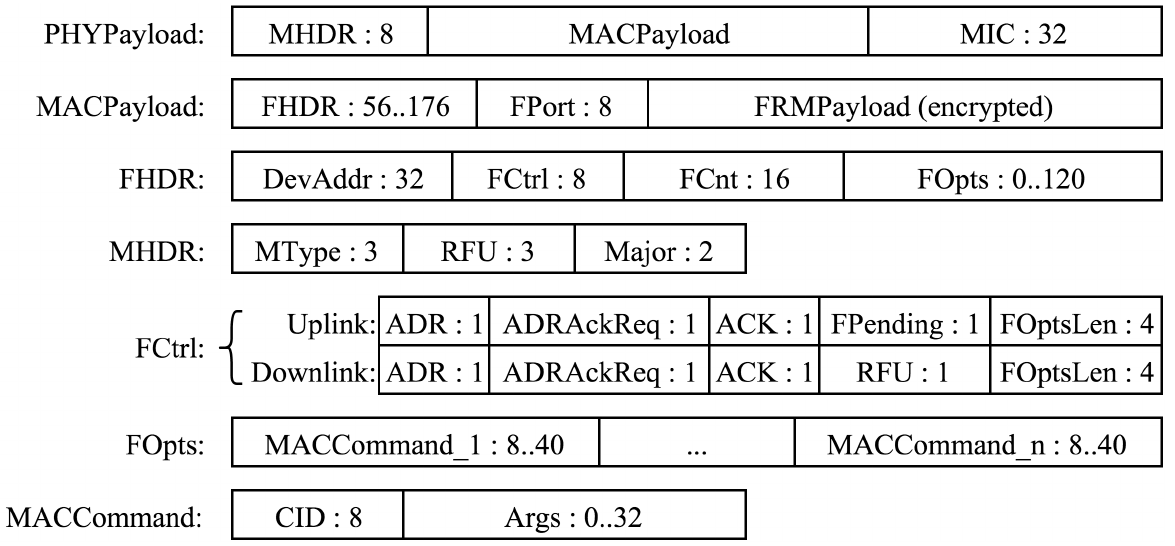
\includegraphics[width=\textwidth]{inc/img/LoRaMACMsgFmt}
  \caption{Формат кадра LoRaWAN. Размеры полей указаны в битах\cite{augustin2016}}
  \label{fig:macframe}
\end{figure}


%%%%%%%%%%%%%%%%%%%%%%%%%%%%%%%%%%%%%%%%%%%%%%%%%%%%%%%%%%%%%%%%%%%%%%%%%%%%%%%%%%%%%%%%%%%%%%%%%%%%%%%%%%%%%%%%

\iffalse

\section{Примеры применения технологии LoRa в концепции Интернета вещей}

\subsection{Умный светильник}

\subsection{Умный счётчик}

%%%%%%%%%%%%%%%%%%%%%%%%%%%%%%%%%%%%%%%%%%%%%%%%%%%%%%%%%%%%%%%%%%%%%%%%%%%%%%%%%%%%%%%%%%%%%%%%%%%%%%%%%%%%%%%%

\section{Преимущества и недостатки в сравнении с другими технологиями}

\subsection{Sigfox}

\subsection{XNB (Стриж)}

\subsection{NB-Fi}

\subsection{LTE/UMTS/GSM}

\fi

%Теперь мы покажем, как изменить нумерацию на «нормальную», если вам этого захочется. Пара команд в начале документа поможет нам.

%\renewcommand{\labelenumi}{\arabic{enumi})}
%\renewcommand{\labelenumii}{\asbuk{enumii})}

%\begin{enumerate}
%\item Изменим нумерацию на более привычную...
%\item ... нарушим этим гост.
%\begin{enumerate}
%\item Но, пожалуй, так лучше.
%\end{enumerate}
%\end{enumerate}

%В заключение покажем произвольные маркеры в списках. Для них нужен пакет \textbf{enumerate}.
%\begin{enumerate}[1.]
%\item Маркер с арабской цифрой и с точкой.
%\item Маркер с арабской цифрой и с точкой.
%\begin{enumerate}[I.]
%\item Римская цифра с точкой.
%\item Римская цифра с точкой.
%\end{enumerate}
%\end{enumerate}

%В отчётах могут быть и таблицы "--- см. табл.~\ref{tab:tabular} и~\ref{tab:longtable}.
%Небольшая таблица делается при помощи \Code{tabular} внутри \Code{table} (последний
%полностью аналогичен \Code{figure}, но добавляет другую подпись).

%\begin{table}[ht]
  %\caption{Пример короткой таблицы с коротким названием}
  %\begin{tabular}{|r|c|c|c|l|}
  %\hline
  %Тело      & $F$ & $V$  & $E$ & $F+V-E-2$ \\
  %\hline
  %Тетраэдр  & 4   & 4    & 6   & 0         \\
  %Куб       & 6   & 8    & 12  & 0         \\
  %Октаэдр   & 8   & 6    & 12  & 0         \\
  %Додекаэдр & 20  & 12   & 30  & 0         \\
  %Икосаэдр  & 12  & 20   & 30  & 0         \\
  %\hline
  %Эйлер     & 666 & 9000 & 42  & $+\infty$ \\
  %\hline
  %\end{tabular}
  %\label{tab:tabular}
%\end{table}

%Для больших таблиц следует использовать пакет \Code{longtable}, позволяющий создавать
%таблицы на несколько страниц по ГОСТ.

%Для того, чтобы длинный текст разбивался на много строк в пределах одной ячейки, надо в
%качестве ее формата задавать \texttt{p} и указывать явно ширину: в мм/дюймах
%(\texttt{110mm}), относительно ширины страницы (\texttt{0.22\textbackslash textwidth})
%и~т.п.

%Можно также использовать уменьшенный шрифт "--- но, пожалуйста, тогда уж во \textbf{всей}
%таблице сразу.

%\begin{center}
  %\begin{longtable}{|p{0.40\textwidth}|c|p{0.30\textwidth}|}
    %\caption{Пример длинной таблицы с длинным названием на много длинных-длинных строк}
    %\label{tab:longtable}
    %\\ \hline
    %Вид шума & Громкость, дБ & Комментарий \\
    %\hline \endfirsthead
    %\subcaption{Продолжение таблицы~\ref{tab:longtable}}
    %\\ \hline \endhead
    %\hline \subcaption{Продолжение на след. стр.}
    %\endfoot
    %\hline \endlastfoot
    %Порог слышимости             & 0     &                                                \\
    %\hline
    %Шепот в тихой библиотеке     & 30    &                                                \\
    %Обычный разговор             & 60-70 &                                                \\
    %Звонок телефона              & 80    & \small{Конечно, это было до эпохи мобильников} \\
    %Уличный шум                  & 85    & \small{(внутри машины)}                        \\
    %Гудок поезда                 & 90    &                                                \\
    %Шум электрички               & 95    &                                                \\
    %\hline
    %Порог здоровой нормы         & 90-95 & \small{Длительное пребывание на более
    %громком шуме может привести к ухудшению слуха}                                        \\
    %\hline
    %Мотоцикл                     & 100   &                                                \\
    %Power Mower                  & 107   & \small{(модель бензокосилки)}                  \\
    %Бензопила                    & 110   & \small{(Doom в целом вреден для здоровья)}     \\
    %Рок-концерт                  & 115   &                                                \\
    %\hline
    %Порог боли                   & 125   & \small{feel the pain}                          \\
    %\hline
    %Клепальный молоток           & 125   & \small{(автор сам не знает, что это)}          \\
    %\hline
    %Порог опасности              & 140   & \small{Даже кратковременное пребывание на
    %шуме большего уровня может привести к необратимым последствиям}                       \\
    %\hline
    %Реактивный двигатель         & 140   &                                                \\
                                 %& 180   & \small{Необратимое полное повреждение
                                 %слуховых органов}                                        \\
    %Самый громкий возможный звук & 194   & \small{Интересно, почему?..}                   \\
  %\end{longtable}
%\end{center}

%%% Local Variables:
%%% mode: latex
%%% TeX-master: "rpz"
%%% End:
